\documentclass[11pt]{article}

\usepackage[margin=1in]{geometry}
\usepackage[T1]{fontenc}
\usepackage[utf8]{inputenc}
\usepackage{lmodern}
\usepackage{amsmath,amssymb}
\usepackage{graphicx}
\usepackage{booktabs}
\usepackage{array}
\usepackage{siunitx}
\usepackage{hyperref}
\usepackage{enumitem}
\usepackage{float}
\usepackage{caption}
\usepackage{longtable}
\usepackage{textcomp}

\hypersetup{
    colorlinks=true,
    linkcolor=black,
    citecolor=black,
    urlcolor=blue,
    pdftitle={Rocket Propulsion Lab - Project Daedalus Technical Report},
    pdfauthor={Marcus Greenan}
}

\setlength{\parskip}{0.6em}
\setlength{\parindent}{0pt}
\captionsetup{font=small}
\setlist[itemize]{leftmargin=*}
\setlist[enumerate]{leftmargin=*}

\graphicspath{
    {../public/projects/rpl-daedalus/}
    {../latex_fix_check/}
}

\begin{document}

\begin{titlepage}
\centering

\vspace*{1.2cm}
\includegraphics[width=0.48\textwidth]{UCSD-Symbol.png}

\vspace{1.4cm}

{\LARGE\bfseries
Rocket Propulsion Lab -- Project Daedalus\\[0.2cm]
Mechanical Design, OpenRocket Simulation,\\[0.2cm]
Preliminary Structural Analysis, and\\[0.2cm]
Subsystem Integration
\par}

\vspace{1.8cm}

{\large Final Technical Report\par}

\vspace{1.2cm}

{\large
Marcus Greenan\\
Structures Lead
\par}

\vspace{1.0cm}

{\large
UC San Diego Rocket Propulsion Laboratory\\
October 2024 -- June 2025
\par}

\vfill

{\large B.S. Mechanical Engineering, Robotics and Controls Specialization\par}
\vspace{0.5cm}
{\small Design target: simulated apogee of approximately \SI{4086}{ft} using an AeroTech G80T motor\par}

\end{titlepage}

\pagenumbering{roman}
\tableofcontents
\newpage

\pagenumbering{arabic}

\section{Abstract}
Project Daedalus was a UC San Diego Rocket Propulsion Laboratory student rocket project focused on designing a compact vehicle that could approach a simulated \SI{4000}{ft} apogee while remaining stable, manufacturable, and recoverable. My role was Structures Lead, with direct work in structural CAD, component interfaces, tolerance checks, manufacturing constraints, and early simulation. The design used an AeroTech G80T motor and an OpenRocket model that predicted an apogee of approximately \SI{4086}{ft}, static stability of 1.23 calibers, peak velocity of \SI{791}{ft/s}, and peak acceleration of \SI{675}{ft/s^2}.

This report documents the mechanical design logic behind the rocket rather than presenting a flight-test result. All altitude, velocity, acceleration, and stability values in this report are simulated or modeled values, not measured flight data. The report focuses on how structural decisions interacted with vehicle mass, center of gravity, center of pressure, avionics packaging, propulsion constraints, recovery deployment, 3D printing, and preliminary structural analysis.

\section{Introduction}
Student rockets are useful engineering projects because they make subsystem coupling unavoidable. A nose cone is not just an aerodynamic surface. It affects mass distribution, recovery deployment, manufacturing, and assembly. Fins are not just stability surfaces. They affect drag, load paths, stiffness, print geometry, and motor-region integration. Project Daedalus forced the team to make these connections early instead of treating each part as an isolated CAD object.

My individual scope was mechanical and structural. I worked on the structural CAD, the nose-cone and body-tube interface, the fin and lower-body region, tolerance decisions, fit behavior, and simulation-informed design checks. I also coordinated with teammates responsible for avionics and propulsion so their hardware could fit inside the vehicle and remain accessible during assembly.

The propulsion, recovery, and avionics systems are discussed because they affected my structural work. They were collaborative team systems rather than solely my individual designs.

\section{System Requirements and Vehicle-Level Targets}
The vehicle-level objective was to create a compact rocket architecture that could approach a simulated \SI{4000}{ft} apogee. The design had to remain stable in the OpenRocket model, package the motor and avionics, support recovery deployment, and be realistic to fabricate with available student-team resources.

\begin{table}[H]
\centering
\caption{Modeled vehicle targets and predicted OpenRocket outputs.}
\small
\begin{tabular}{lll}
\toprule
Parameter & Value & Interpretation \\
\midrule
Vehicle length & \SI{25}{in} & Overall modeled rocket length \\
Maximum diameter & \SI{1.5}{in} & Primary vehicle envelope \\
Modeled mass & \SI{1.038}{lb} / \SI{0.471}{kg} & OpenRocket vehicle mass with motor \\
Selected motor & AeroTech G80T & Design motor used in the model \\
Simulated static stability & 1.23 calibers & OpenRocket predicted stability margin \\
Simulated apogee & Approx. \SI{4086}{ft} / \SI{1245}{m} & Modeled altitude prediction \\
Simulated peak velocity & \SI{791}{ft/s} / \SI{241}{m/s} & Modeled maximum vertical velocity \\
Simulated peak acceleration & \SI{675}{ft/s^2} / \SI{205.74}{m/s^2} & Modeled maximum vertical acceleration \\
Simulated time to apogee & Approx. \SI{14.1}{s} & Modeled ascent timing \\
\bottomrule
\end{tabular}
\end{table}

\section{Vehicle Architecture}
The rocket architecture was constrained by a narrow \SI{1.5}{in} diameter body, a \SI{25}{in} total length, and the need to package motor, recovery hardware, avionics, wiring, and structural interfaces inside a small volume. The structure could not be designed separately from these systems because any change to component position shifted the center of gravity, center of pressure relationship, and recovery packaging.

\begin{figure}[H]
    \centering
    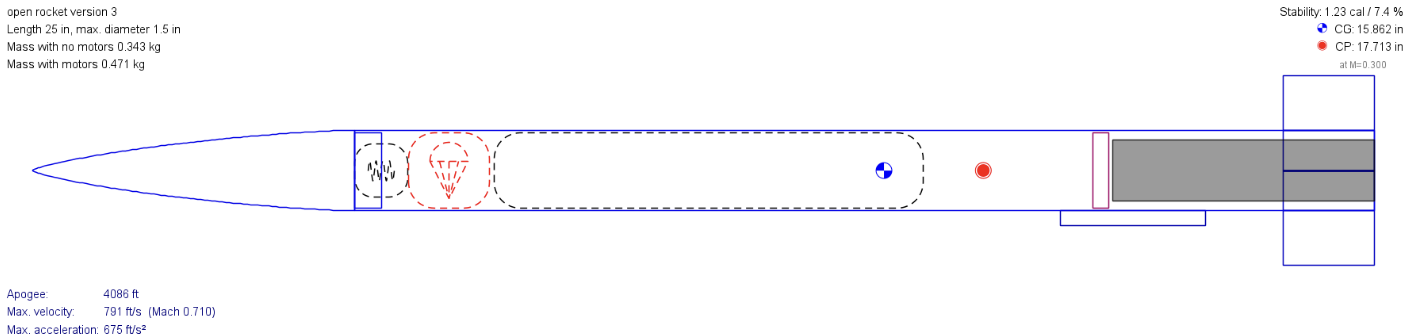
\includegraphics[width=0.95\linewidth]{openrocket-vehicle-model.png}
    \caption{OpenRocket vehicle model showing geometry, internal component placement, modeled center of gravity, and modeled center of pressure.}
    \label{fig:openrocket-vehicle}
\end{figure}

\begin{table}[H]
\centering
\caption{Subsystem architecture and structural-interface relevance.}
\small
\begin{tabular}{p{0.22\linewidth}p{0.68\linewidth}}
\toprule
Subsystem & Notes \\
\midrule
Body structure & \SI{25}{in} total vehicle length, \SI{1.5}{in} maximum diameter, approximately \SI{19}{in} body tube, approximately \SI{1.4}{in} inner diameter, and an engine block separating the motor and avionics regions. \\
Fin assembly & Four fins with approximately \SI{1.7}{in} root chord, approximately \SI{1.02}{in} height, airfoil-style cross section, and integration with a printed fin-can or sleeve structure. \\
Recovery & \SI{24}{in} ripstop nylon parachute, nose-cone deployment, approximately \SI{10.5}{ft/s} predicted ground-contact velocity, and deployment near simulated apogee. \\
Propulsion & AeroTech G80T motor, \SI{133}{N.s} total impulse, approximately \SI{78}{N} average thrust, and approximately \SI{1.71}{s} burn duration. \\
Avionics & Arduino Pro Mini, BMP280 pressure sensor, MPU6050 inertial sensor, SD-card data logging, wiring, mounting hardware, and \SI{7.4}{V} LiPo battery. \\
\bottomrule
\end{tabular}
\end{table}

\section{Mechanical and Structural Design}
My structural work focused on keeping the CAD realistic as the vehicle architecture changed. That meant reviewing how the nose cone, body tube, fin assembly, avionics bay, motor region, recovery hardware, and printed interfaces fit together. The most important mechanical problem was not a single isolated component. It was making sure parts that looked correct in CAD could still assemble, retain, separate, and leave enough space for adjacent systems.

Structural decisions were checked against four recurring constraints: mass, stiffness, fit, and access. Adding material improved rigidity but changed the center of gravity. Tightening a fit improved retention but could interfere with nose-cone deployment. Moving electronics improved access but changed mass distribution. These tradeoffs made OpenRocket and preliminary structural simulation useful early filters before fabrication.

\section{Nose-Cone Design}
The nose cone had several jobs at once. It defined the leading aerodynamic geometry, added structural mass near the front of the vehicle, connected to the body tube, and separated as part of the recovery sequence. The Von Kármán profile gave the team a practical aerodynamic shape for the available length and diameter while staying compatible with in-house 3D printing.

\begin{table}[H]
\centering
\caption{Nose-cone design parameters.}
\small
\begin{tabular}{ll}
\toprule
Parameter & Value \\
\midrule
Length & \SI{6}{in} \\
Maximum diameter & \SI{1.5}{in} \\
Fineness ratio & 4.0 \\
Profile & Haack Series, Von Kármán, C = 0 \\
Material & PLA \\
Infill & 100\% \\
Manufacturing & In-house 3D printing \\
Shoulder outer diameter & \SI{1.4}{in} \\
Shoulder inner diameter & \SI{1.3}{in} \\
Shoulder height & \SI{0.5}{in} \\
\bottomrule
\end{tabular}
\end{table}

Using high infill increased rigidity, but it also increased forward mass. That mass affected the vehicle's center of gravity, which meant the nose-cone design had to be evaluated in the context of the complete OpenRocket model. The shoulder used a friction-fit connection with the body tube. The fit needed to remain secure during handling and ascent while still allowing the recovery system to separate the nose cone near apogee.

The key design takeaway is that the nose cone was simultaneously an aerodynamic component, a printed structural part, a mass-distribution input, and a recovery-system interface.

\section{Manufacturing and Tolerance Considerations}
Manufacturing constraints affected the design before any part was printed. The rocket used printed structural components and a small body diameter, so clearance decisions mattered. A part that was dimensionally acceptable in CAD could still create problems if printer tolerance, wall geometry, infill, or friction-fit behavior was not considered.

The most important tolerance concern was the relationship between retention and deployment. The nose-cone shoulder needed enough friction to remain assembled before deployment, but too much interference could prevent separation during recovery. Similar logic applied to the fin-can and motor-region interfaces: stiffness and retention had to be balanced against added mass, assembly difficulty, and the risk of damaging nearby components.

\section{Avionics Packaging and Mechanical Interfaces}
The avionics package affected the structural design even though my primary role was mechanical. The Arduino, pressure sensor, inertial sensor, SD-card module, battery, wiring, and mounting hardware all had to fit within the available internal diameter. Mechanical design decisions had to preserve enough room for wiring, sensor placement, assembly, and removal.

I regularly communicated with the electrical team to understand what space they needed and where mechanical access mattered. That communication helped prevent structural changes from creating packaging or serviceability problems for avionics.

\begin{figure}[H]
    \centering
    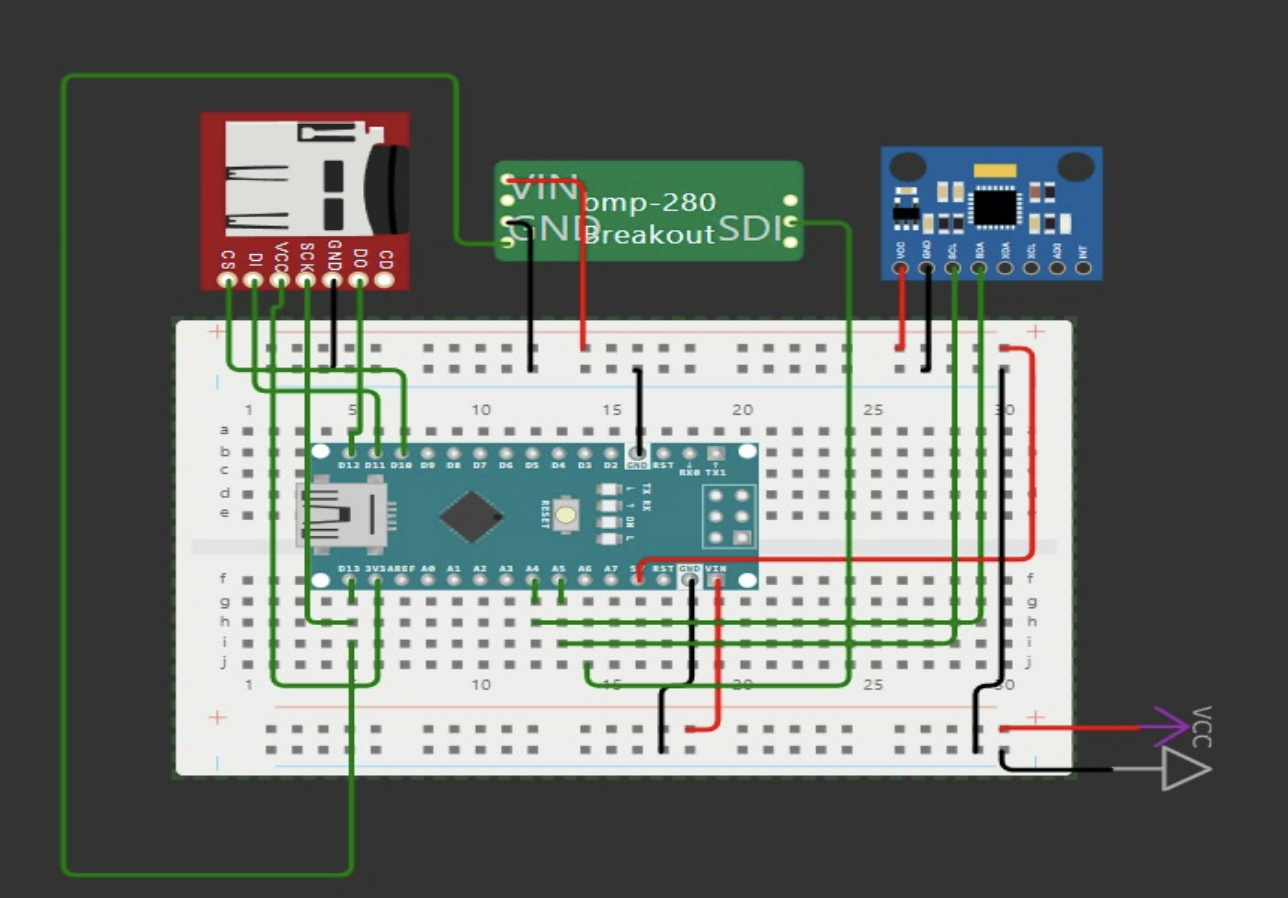
\includegraphics[width=0.86\linewidth]{avionics-layout.png}
    \caption{Early avionics circuit and sensor architecture used to define packaging and mechanical-interface requirements.}
    \label{fig:avionics}
\end{figure}

\section{OpenRocket Modeling and Predicted Flight Performance}
OpenRocket was used to evaluate vehicle geometry, component placement, mass distribution, center of gravity, center of pressure, static stability, predicted apogee, velocity, acceleration, and time to apogee. The model helped the team see how structural changes affected the complete vehicle.

I used these results as design guidance rather than treating the simulation as a substitute for physical validation. A change that improved one component could shift the center of gravity, change stability, add drag, or reduce predicted altitude. OpenRocket helped identify weak concepts and compare alternatives before fabrication.

\begin{table}[H]
\centering
\caption{Selected OpenRocket prediction outputs.}
\small
\begin{tabular}{ll}
\toprule
OpenRocket output & Predicted value \\
\midrule
Simulated apogee & Approx. \SI{4086}{ft} \\
Simulated static stability & 1.23 calibers \\
Simulated time to apogee & Approx. \SI{14.1}{s} \\
Simulated peak velocity & \SI{791}{ft/s} \\
Simulated peak acceleration & \SI{675}{ft/s^2} \\
\bottomrule
\end{tabular}
\end{table}

\begin{figure}[H]
    \centering
    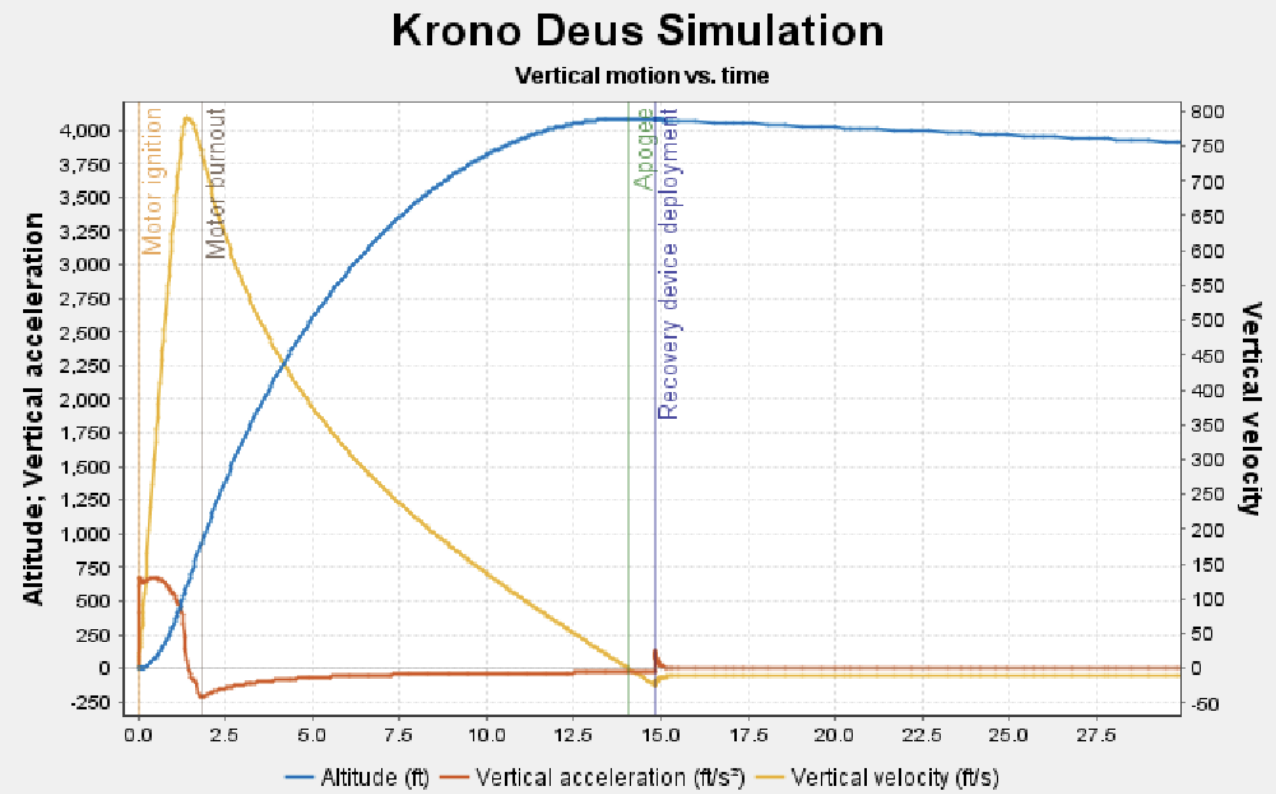
\includegraphics[width=0.94\linewidth]{openrocket-flight-simulation.png}
    \caption{OpenRocket prediction of altitude, vertical velocity, and vertical acceleration over the modeled flight. These values are simulated and should not be read as measured flight data.}
    \label{fig:openrocket-flight}
\end{figure}

\section{Qualitative Flow and Pressure Review}
The flow simulation gave the team an early qualitative view of the pressure field and flow paths around the rocket geometry. It helped us identify areas of the vehicle worth examining and communicate how the external geometry interacted with the surrounding flow.

This result should be treated as an exploratory design study, not validated computational fluid dynamics. The project materials do not document enough about the mesh, boundary conditions, turbulence model, convergence behavior, or experimental correlation to support stronger CFD claims.

\begin{figure}[H]
    \centering
    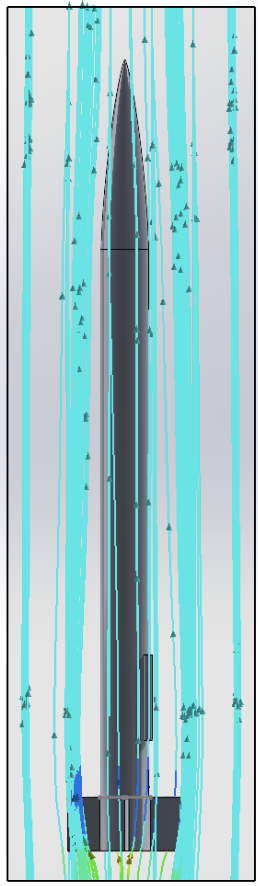
\includegraphics[height=0.72\textheight]{flow-simulation.png}
    \caption{Qualitative flow and pressure visualization around the rocket geometry. Cooler colors indicate lower displayed pressure and warmer colors indicate higher displayed pressure.}
    \label{fig:flow}
\end{figure}

\section{Preliminary Structural Simulation Review}
The structural simulations were used as preliminary design checks rather than formal qualification. They provided a way to inspect where deformation, strain, and stress concentrated under the modeled load before the team committed to fabrication.

The documented loading case applied approximately \SI{39.25}{lb} to the modeled structure. The visual results helped the team review the body and fin region for concerning behavior and identify geometry that deserved closer attention. This report does not claim a factor of safety, yield-strength comparison, or pass/fail qualification because those values are not documented in the supplied source material.

\begin{figure}[H]
    \centering
    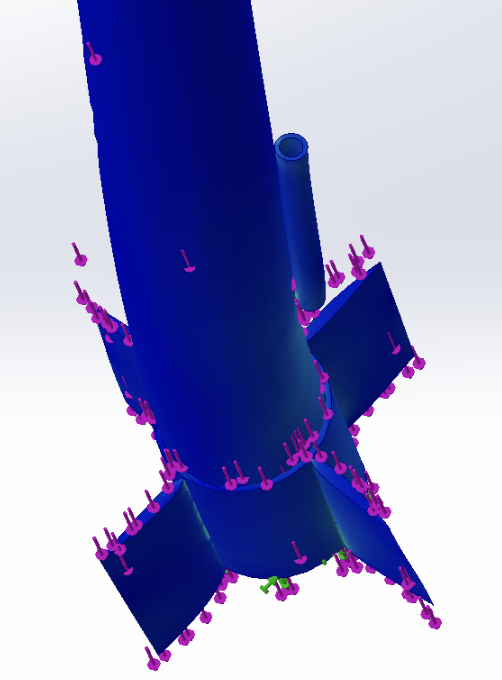
\includegraphics[height=0.62\textheight]{pressure-stress.png}
    \caption{Von Mises stress visualization used as an early structural design check under the documented modeled loading case.}
    \label{fig:stress}
\end{figure}

\section{Design Process}
\begin{enumerate}
    \item \textbf{Requirements:} Defined the approximate altitude target, vehicle envelope, stability needs, recovery approach, motor constraints, and manufacturing limits.
    \item \textbf{Concept development:} Created and reviewed early CAD for the nose cone, body structure, fins, avionics bay, and subsystem interfaces.
    \item \textbf{Simulation:} Used OpenRocket and preliminary structural studies to review stability, predicted performance, and structural behavior.
    \item \textbf{Integration:} Coordinated with propulsion and avionics teammates as packaging and hardware requirements developed.
    \item \textbf{Refinement:} Adjusted geometry, fit, material use, and component placement based on integration and manufacturing constraints.
    \item \textbf{Fabrication and testing support:} Supported fabrication planning, physical assembly, and team testing activities.
\end{enumerate}

\section{Engineering Tradeoffs}
\subsection{Aerodynamics versus Manufacturability}
The external geometry influenced drag, but the part still had to fit the available printer, print reliably, and connect to the body tube without excessive post-processing.

\subsection{Stiffness versus Mass}
Increasing material, infill, or thickness improved rigidity but also changed total vehicle mass and shifted the center of gravity.

\subsection{Retention versus Deployment}
The nose-cone interface needed enough friction to remain assembled before deployment without preventing the recovery system from separating it.

\subsection{Packaging versus Stability}
Moving the motor, avionics, battery, recovery hardware, or printed components changed mass distribution and therefore affected both mechanical integration and aerodynamic stability.

\section{Conclusion}
Project Daedalus taught me to connect CAD, simulation, manufacturing, and subsystem communication. My strongest contribution was not a single isolated component. It was making structural decisions while accounting for how the complete rocket needed to assemble, remain stable, package its hardware, and support recovery.

The project changed how I think about mechanical design. A part can look correct in isolation and still cause problems when tolerances, manufacturing limits, wiring, mass distribution, recovery motion, and neighboring subsystems become real. I learned to check interfaces earlier, use simulation to eliminate weak concepts before fabrication, and evaluate structural decisions in the context of the complete vehicle.

\end{document}
